\documentclass[supercite]{HustGraduPaper}
%进行个人信息设置
\title{生物信息学上机实验} %论文题目
\author{张皓鸿} %作者姓名
\date{\today} %日期,默认当日
\school{生命科学与技术学院} %院系名称
\classnum{登峰1901班} %专业班级
\stunum {U201912537} %学号

%添加自己要用的其他宏包
\usepackage{xltxtra}
\usepackage{bm}
\usepackage{algorithmicx}
\usepackage{float}
\usepackage{hyperref}
\hypersetup{
	colorlinks=true,
	linkcolor=cyan,
	filecolor=blue,
	urlcolor=blue,
	citecolor=blue,
}
\usepackage{graphicx}

\begin{document}
	%生成标题页 \maketitle[可选参数]
	%可选参数:
	%logo color=green/black 华中科技大学字样的颜色,绿色或者黑色,默认绿色
	%line length=12em 填写信息处横线的长度,默认12em
	%line font=huawenzhongsong 填写信息的字体,默认huawenzhongsong
	\maketitle[logo color=black]

	\clearpage %结束上一页
	\tableofcontents
	\clearpage%结束上一页
	\pagenumbering{arabic} %正文页码为阿拉伯数字

	%正文内容从这里开始
	\section{基因组分析}
	\subsection{总结β属冠状病毒和SARS-CoV-2(2019-nCoV)的主要特点}
  \paragraph{}\label{subpara:subpara}1、都是RNA病毒
	\paragraph{}\label{subpara:subpara}2、 冠状病毒的s蛋白分为两个功能单元S1和S2。S1通过与宿主受体结合促进病毒感染。它包括两个结构域,n端结构域和c端RBD结构域,它们通过s蛋白与ACE2受体结合而感染人类。

  \subsection{编写并运行example4-1.pl}
	\paragraph{}编写的example4-1.pl如下
  \begin{figure}[H]
		\centering
  	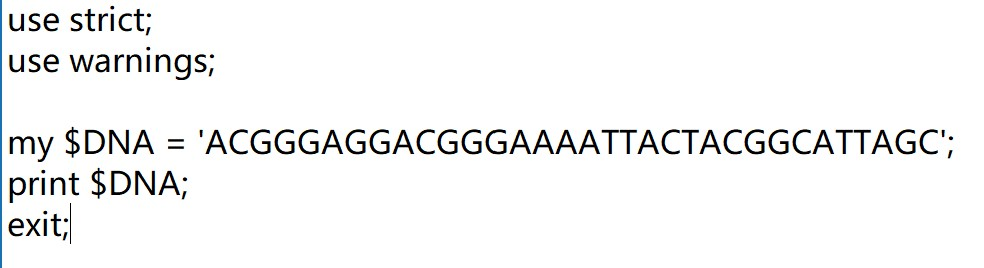
\includegraphics{./material/practice1/perl_1.jpg}
  	\caption{example4-1.pl}
  \end{figure}

	\subsection{SARS-CoV-2的基因组序列}
	\paragraph{}\label{subpara:subpara}得到新冠病毒基因的fasta文件后,通过如下perl程序得到其互补序列。
	\begin{figure}[H]
		\centering
		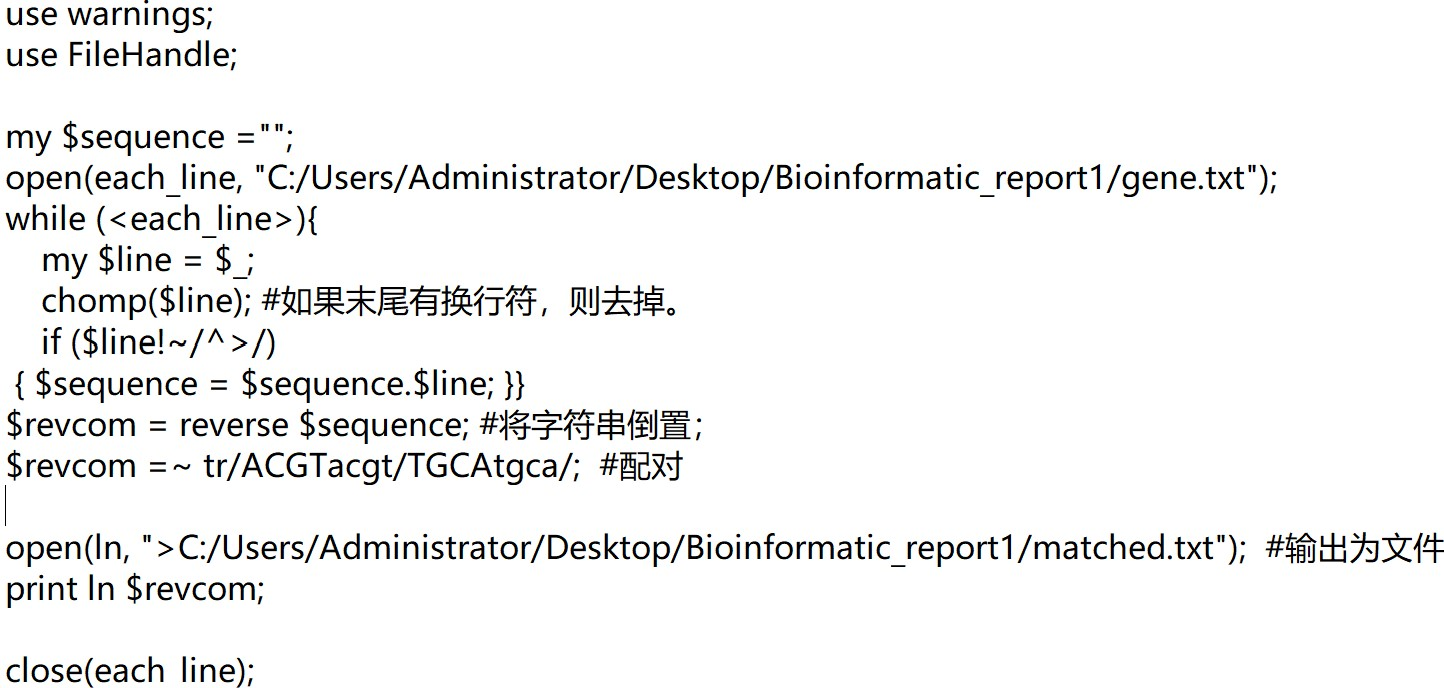
\includegraphics{./material/practice1/perl_2.jpg}
		\caption{gene\_match.pl}
	\end{figure}

  \subsection{SARS-CoV-2潜在编码序列的预测}
	\paragraph{}\label{subpara:subpara}预测开放阅读框如下
	\begin{figure}[H]
		\centering
		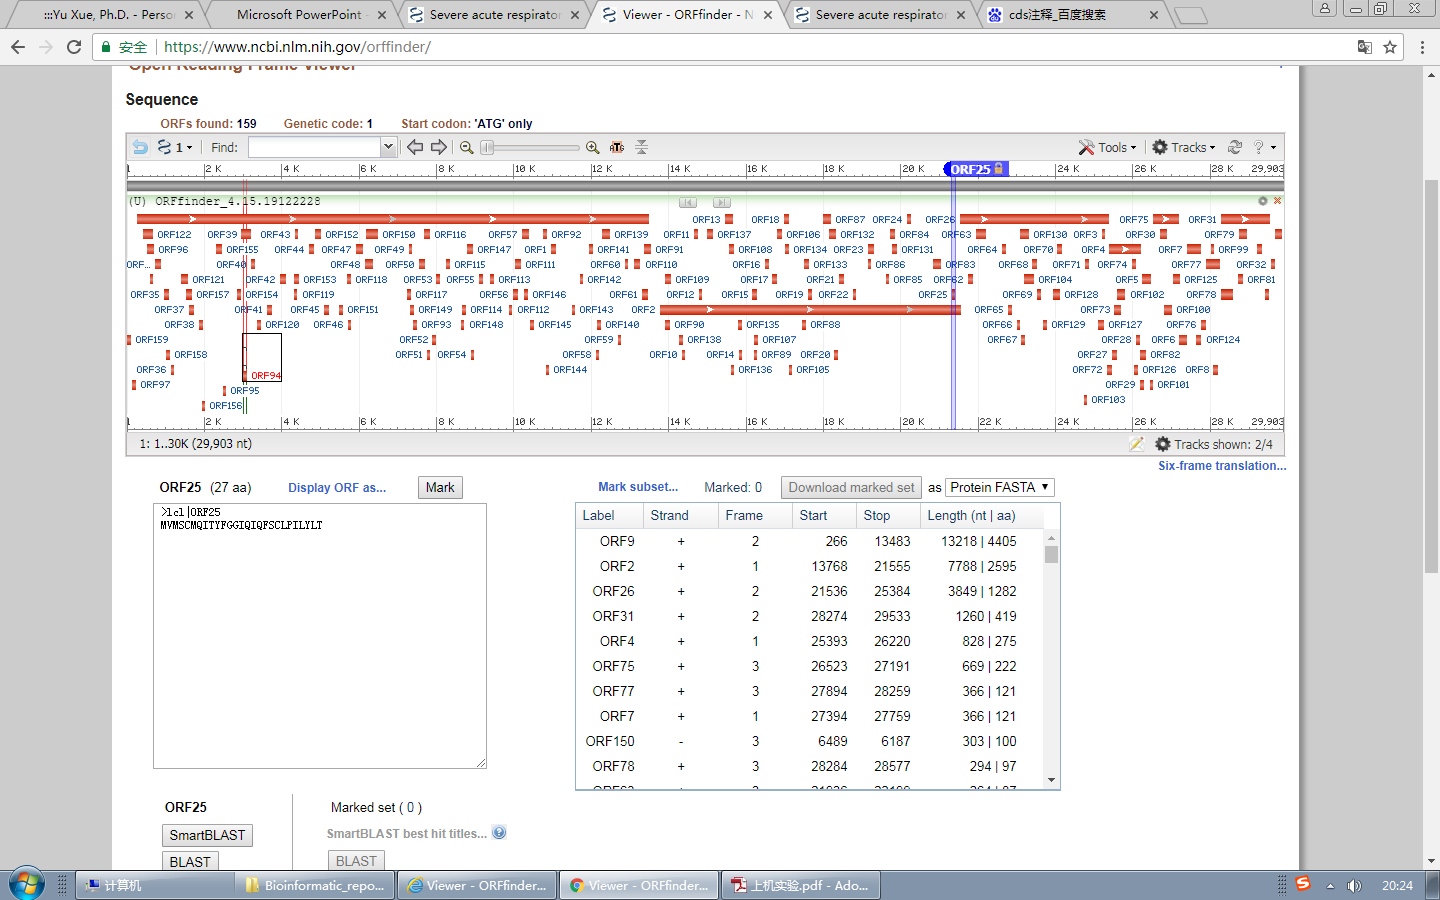
\includegraphics[width=1\textwidth]{./material/practice1/ORF.PNG}
    \caption{ORF\_prediction.PNG}
  \end{figure}

	\paragraph{}\label{subpara:subpara}CDS注释如下
	\begin{figure}[H]
		\centering
		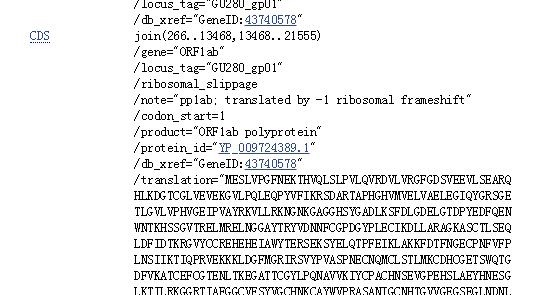
\includegraphics[width=1\textwidth]{./material/practice1/CDS.png}
		\caption{CDS\_annotation.PNG}
	\end{figure}
	\paragraph{}\label{subpara:subpara}通过比较预测的ORF与CDS注释可以发现,预测的ORF几乎占据了整段基因,但实际CDS仅为其中的一部分,说明基因并不是整段表达的。
  \subsection{发现与SARS-CoV-2同源的冠状病毒}
	\begin{table}[H]
		\begin{center}
			\begin{tabular}{|cccc|}
				\hline
				MT461669.1 & MT108784.1 & HG994854.1 & HG994852.1 \\
				HG994857.1 & HG994855.1 & MT461671.1 & MT461670.1 \\
        MN996532.2 & HG994858.1 & HG994859.1 &
        HG994856.1 \\
				HG994853.1 & MT121216.1 & MW703458.1 & MT040335.1 \\
				MT040333.1 & MT072864.1 & MT040334.1 & MT040336.1 \\ \hline
			\end{tabular}
			\caption{20个SARS-CoV-2的同源冠状病毒的序列号}
		\end{center}
	\end{table}
  \subsection{插入片段分析}
	  \paragraph{}\label{subpara:subpara}使用megablast, dimegablast, blastn搜索结果如下
		\begin{figure}[H]
			\centering
			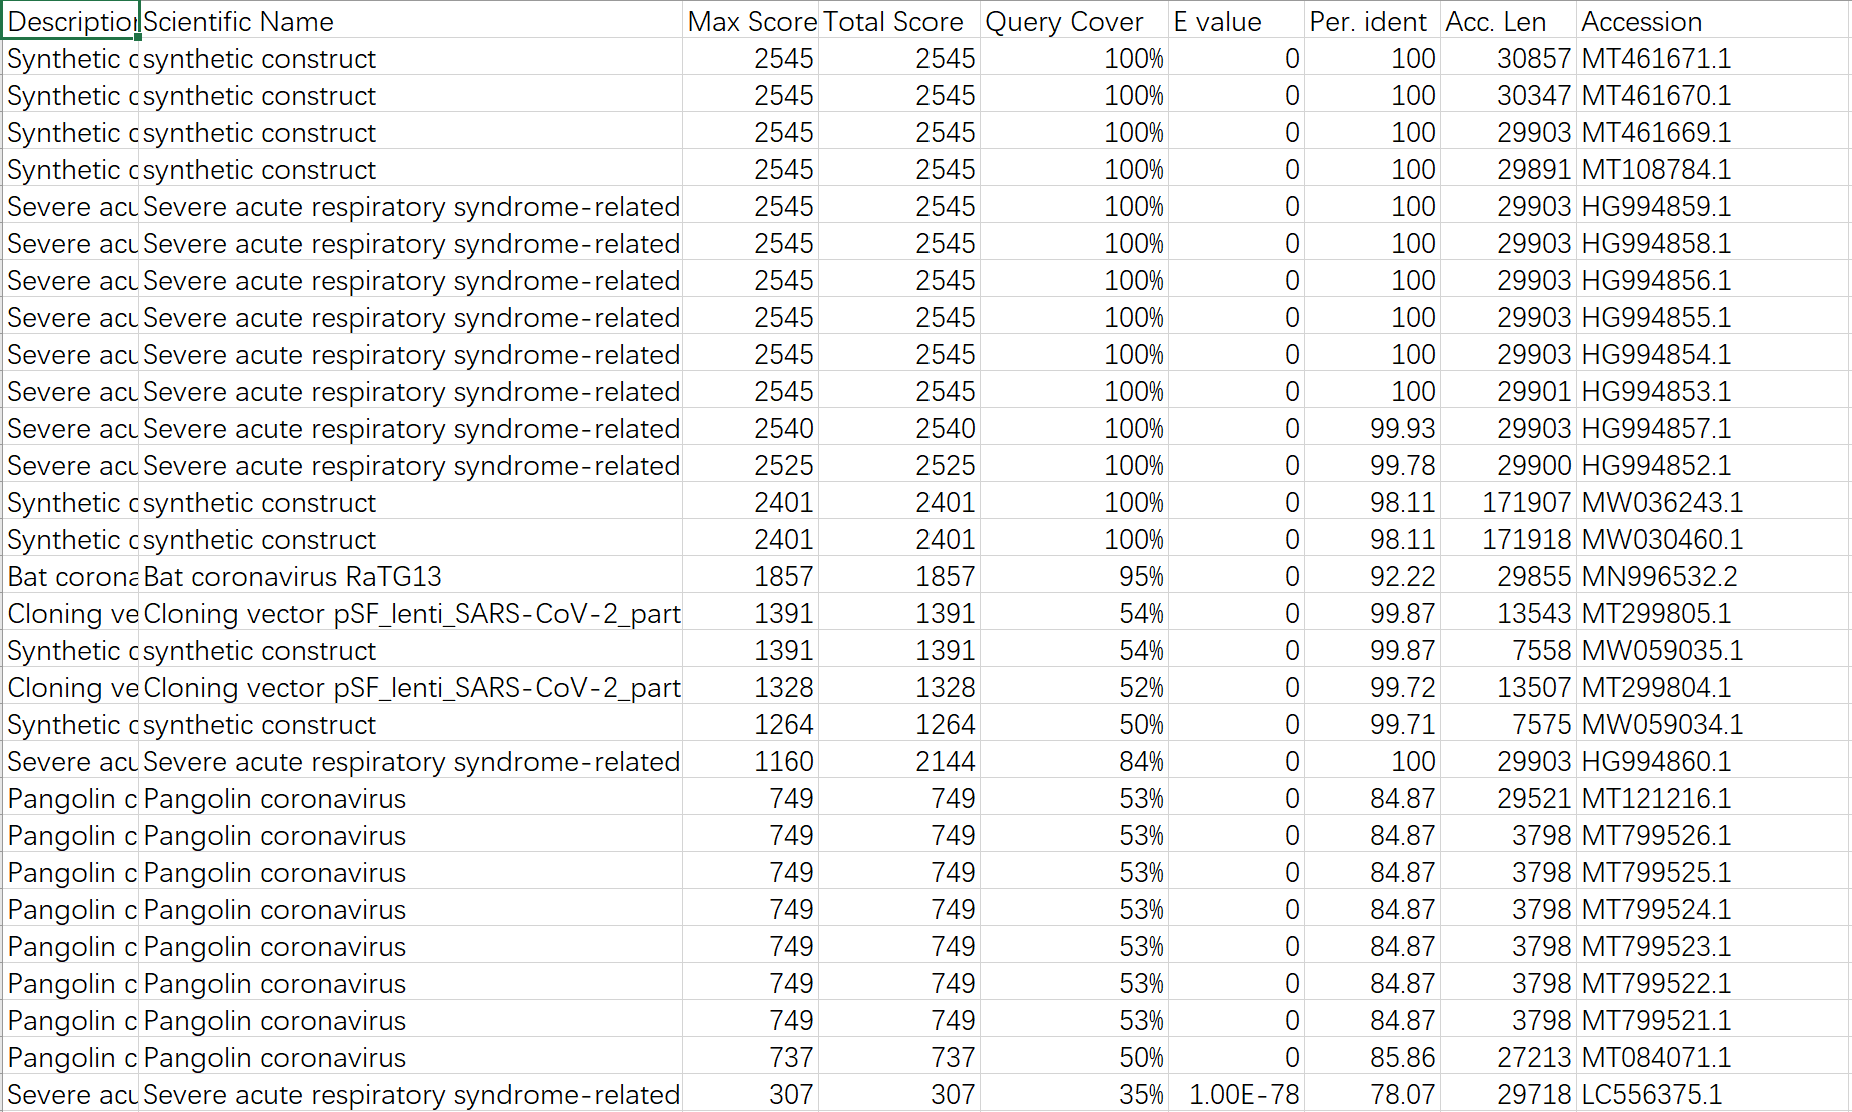
\includegraphics[width=1\textwidth]{./material/practice1/megablast_result.png}
			\caption{megablast\_result.PNG}
		\end{figure}
		\begin{figure}[H]
			\centering
			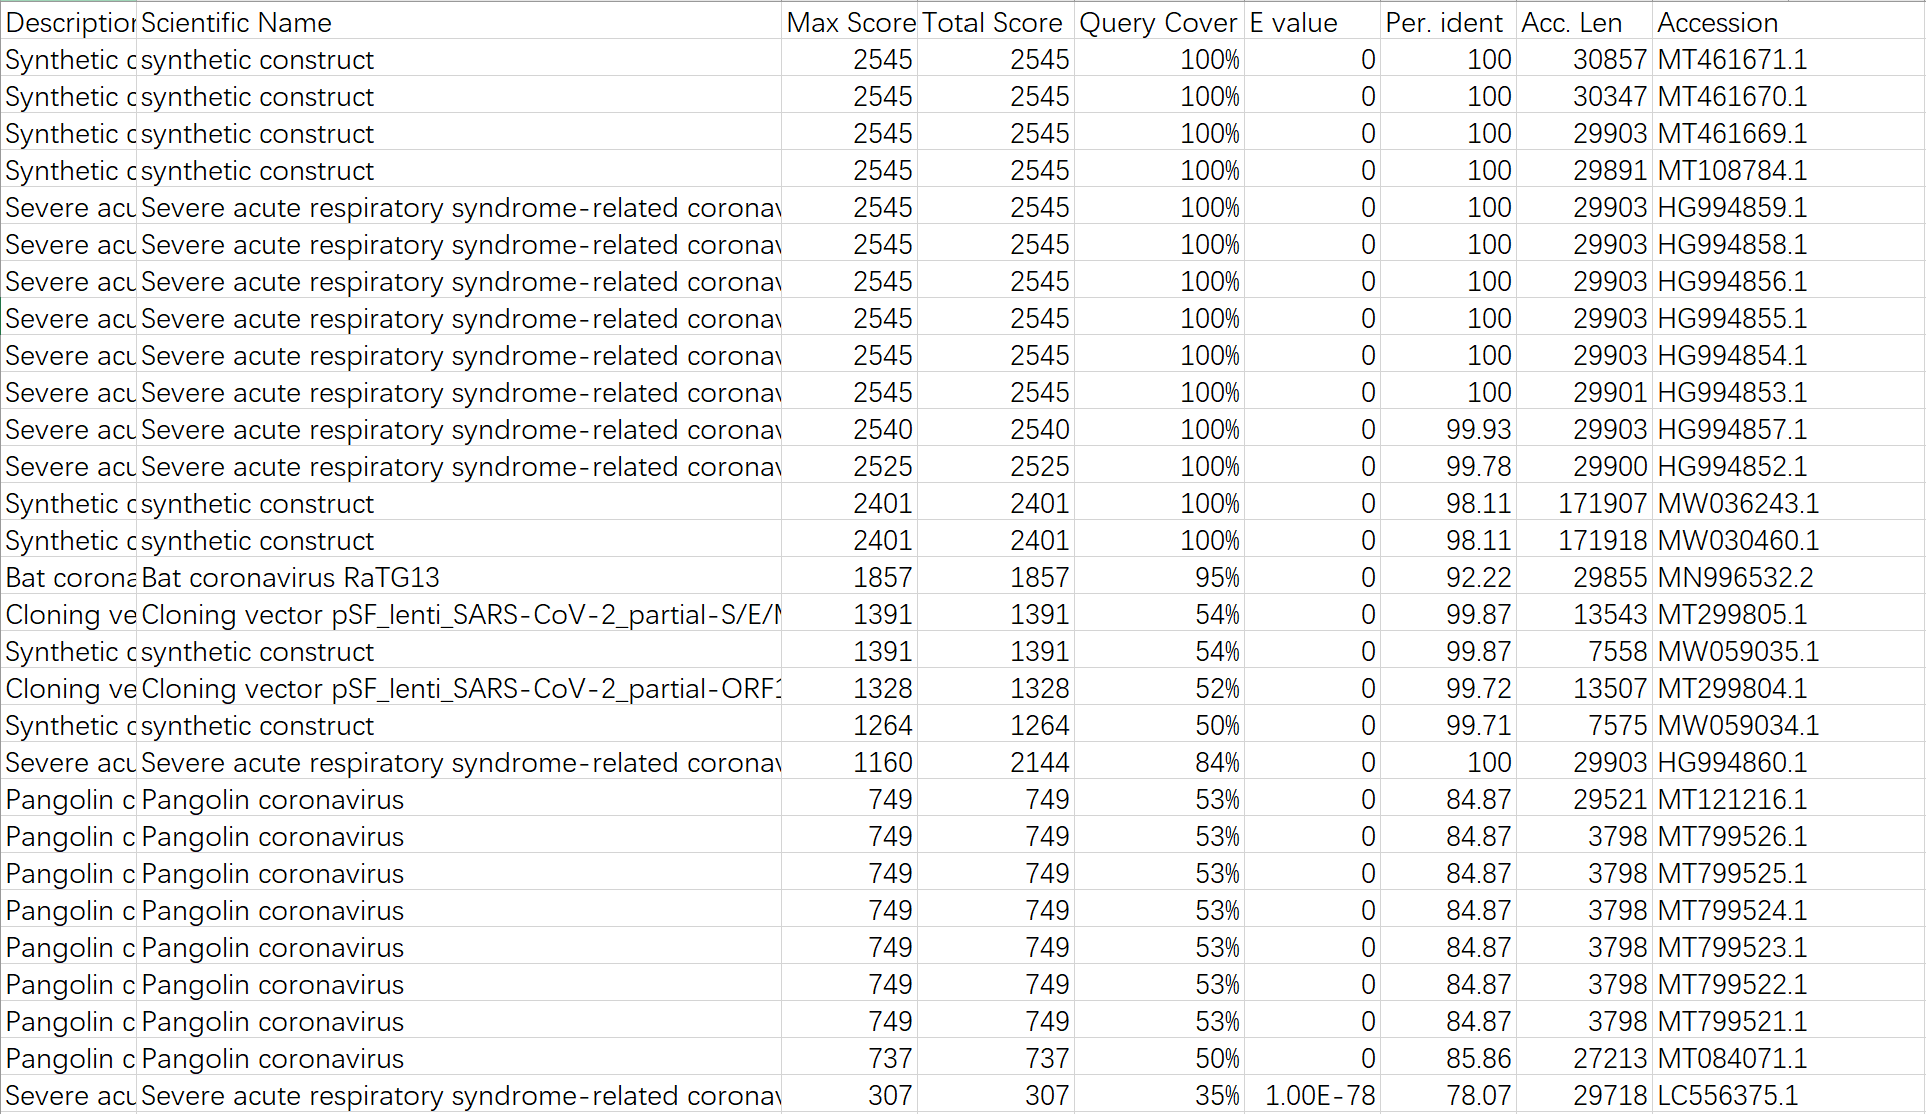
\includegraphics[width=1\textwidth]{./material/practice1/dimegablast_result.png}
			\caption{dimegablast\_result.PNG}
		\end{figure}
		\begin{figure}[H]
			\centering
			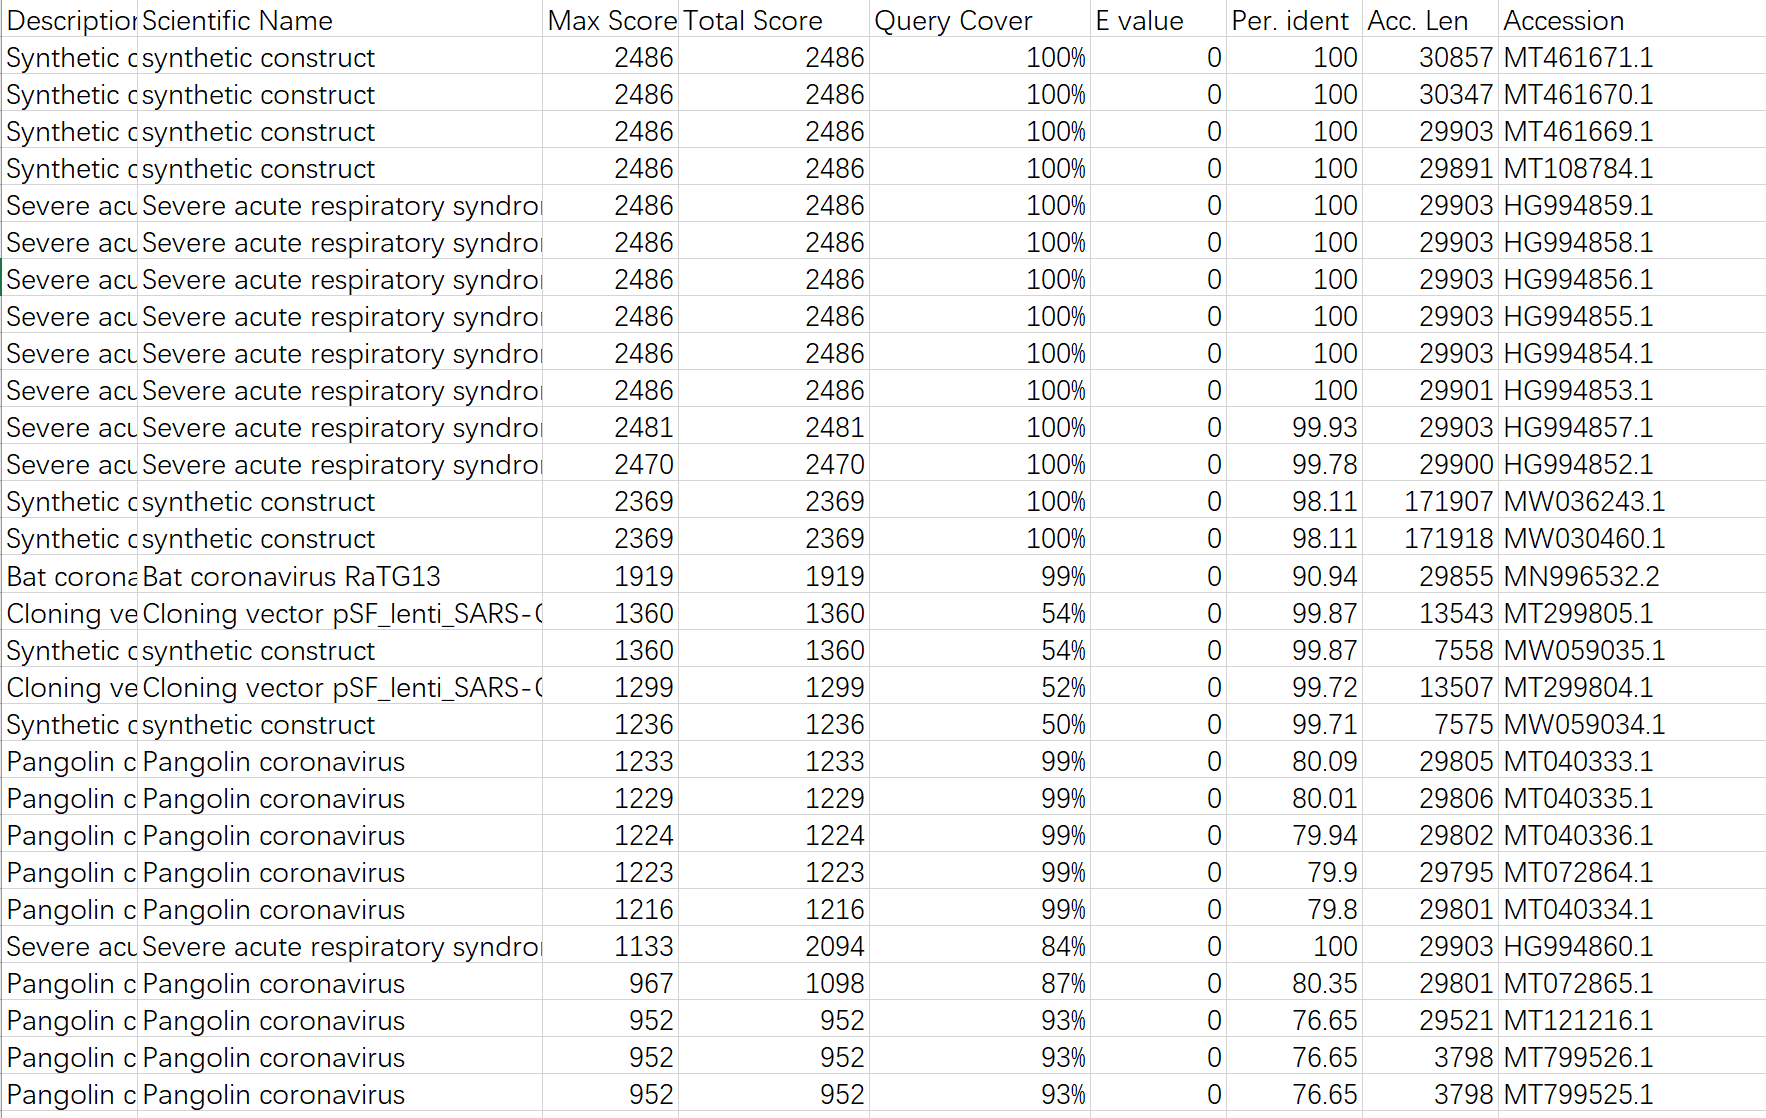
\includegraphics[width=1\textwidth]{./material/practice1/blastn_result.png}
			\caption{blastn\_result.PNG}
		\end{figure}
		\paragraph{}\label{subpara:subpara}可以看出megablast的结果较少,但使用dimegablast与blastn允许错配后,可用结果变多,故该基因在冠状病毒中保守,不为人工插入序列。

	\section{序列分析}
	\subsection{INS1378与pShuttle-SN载体的相似性}
    \paragraph{}\label{subpara:subpara}Global Align与EMBOSS Water比对结果如下
		\begin{figure}[H]
			\centering
			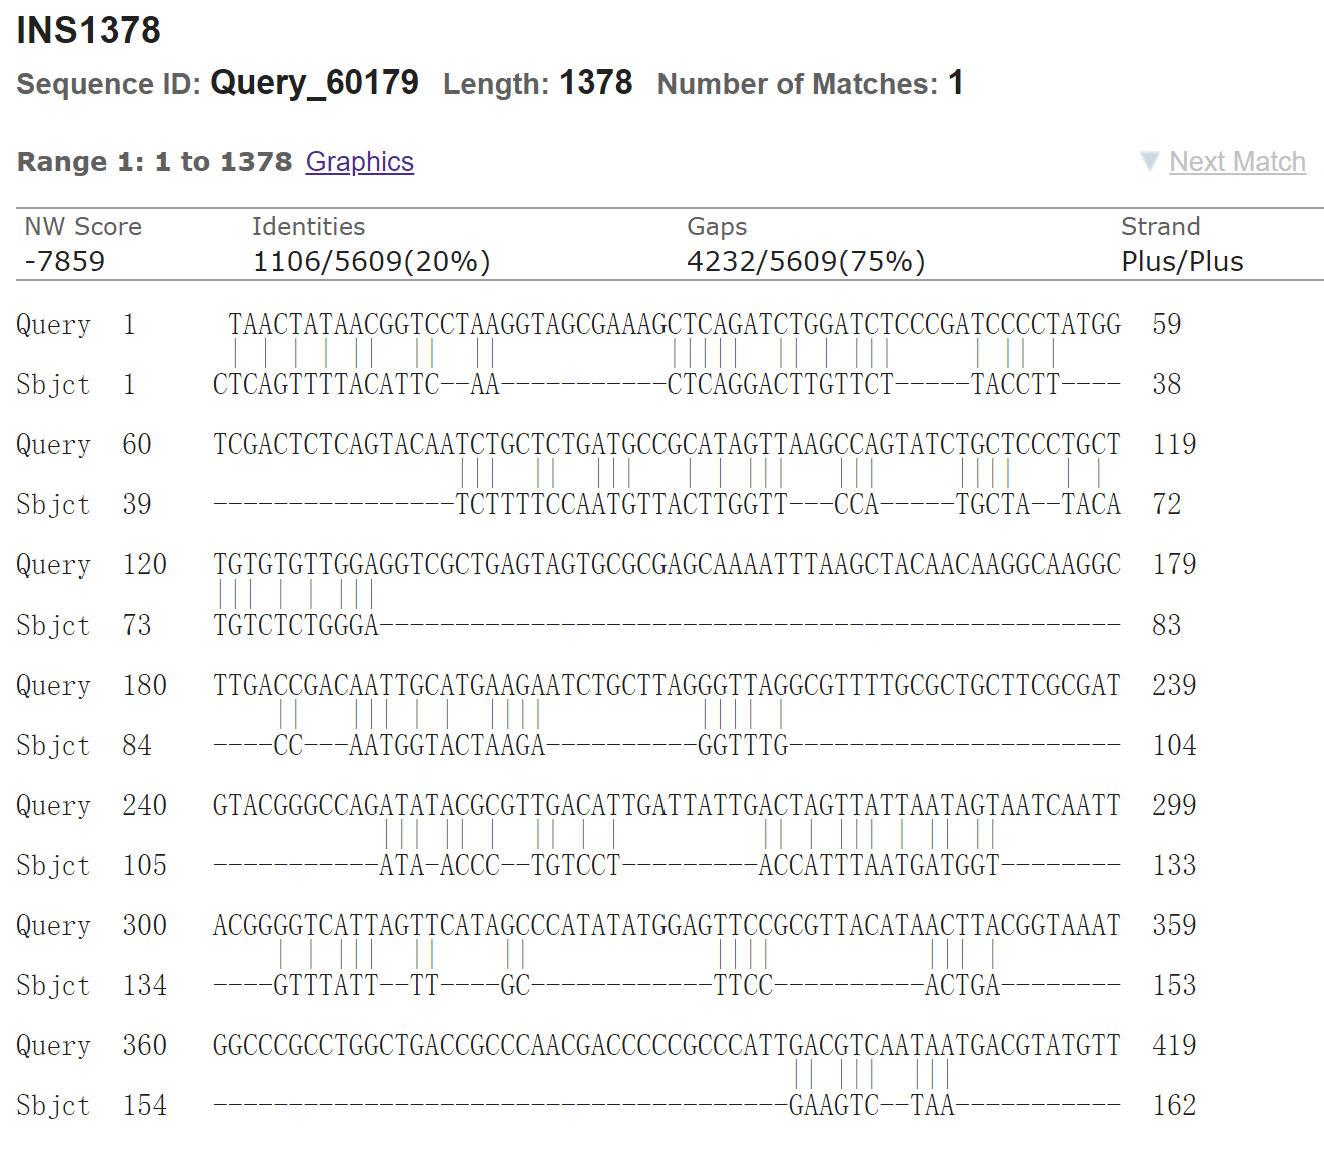
\includegraphics[width=1\textwidth]{./material/practice2/global_align.png}
			\caption{global\_align.PNG}
		\end{figure}
		\begin{figure}[H]
			\centering
			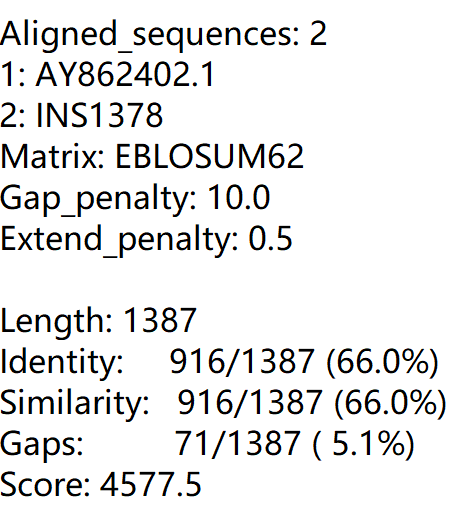
\includegraphics[width=1\textwidth]{./material/practice2/emboss_water.png}
			\caption{EMBOSS\_Water.PNG}
		\end{figure}
		\paragraph{}\label{subpara:subpara}Global Align使用的是Needleman Wunsh算法,出现负分,且结果序列gap较多;EMBOSS Water使用Smith Waterman算法,出现负分则记为零分,结果序列gap较少。
	\subsection{SARS-CoV-2的蛋白质序列}

	\subsection{等电点与分子量分析}
	\begin{table}[H]
  \begin{center}
    \begin{tabular}{|l|c|r|} % <-- Alignments: 1st column left, 2nd middle and 3rd right, with vertical lines in between
			\hline
      \textbf{序号} & \textbf{等电点pI} & \textbf{分子量Mw}\\
      \hline
			  CDS\_1 & 6.32 & 794057.79\\
        CDS\_2 & 6.04 & 489988.91\\
        CDS\_3 & 6.24 & 141178.47\\
        CDS\_4 & 5.55 & 31122.94\\
        CDS\_5 & 8.57 & 8365.04\\
        CDS\_6 & 9.51 & 25146.62\\
        CDS\_7 & 4.60 & 7272.54\\
  	    CDS\_8 & 8.23 & 13744.17\\
  	    CDS\_9 & 4.17 & 5180.27\\
  	    CDS\_10 & 5.42 & 13831.01\\
  	    CDS\_11 & 10.07 & 45625.70\\
  	    CDS\_12 & 7.93 & 4449.23\\ \hline
    \end{tabular}
		    \caption{编码蛋白等电点与分子量}
  \end{center}
\end{table}
	\subsection{功能结构域分析}

	\subsection{细胞亚定位分析}
\section{进化分析}
\section{Spike蛋白分析}

\end{document}
